\newpage
\section{DESARROLLO Y ANÁLISIS DE RESULTADOS}

A continuación se muestran los métodos de desarrollo utilizados para resolver cada uno de los problemas planteados, así como la funciones utilizadas, el método de operación a partir de diagramas de flujo y los resultados obtenidos:

\subsection{Desarrollo de la solución}

A continuación podrá consultarse una descripción de alto nivel de cada una de las funciones implementadas para conseguir los objetivos del presente laboratorio: 

\subsubsection{Función \texttt{init()}}
Esta función se encarga de configurar e inicializar los registros necesarios para permitir el funcionamiento esperado del microcontrolador. Al inicio de la función, se le da valor a alguna variables globales y se habilitan las interrupciones globales haciendo el llamado de la función \texttt{sei()}. Además, se configuran los pines del puerto B que se utilizarán, tanto su estado como su modo. Lo siguiente es la configuración de la interrupción externa INT0, la cual permite controla el cruce a través de un pulsador. Finalmente se configura el temporizador 0 utilizando el modo de \textit{Clear Timer on Compare Match}. 

\subsubsection{Rutina de interrupción externa}
Esta función se activa cuando se produce una interrupción externa en el microcontrolador, en este caso específico, cuando ocurre una interrupción en el pin INT0. El objetivo de esta función es almacenar el una variable global llamada \texttt{btn\_pushed} un 1, cuando el botón conectado al pin PD2 (pin 6) ha sido presionado. Lo anterior permite la activación de la máquina de estados más adelante. 

\subsubsection{Rutina de interrupción de temporizador}
Esta función se activa cada vez que ocurre un CTC y permite controlar el tiempo del programa, ya que tras \textit{n} (en este caso es 60) comparaciones exitosos, suma una unidad a la variable global de segundos. Lo anterior permite que la máquina de estados realice las transiciones en los momentos adecuados. Asimismo, hace posible los parpadeos de los estados en los que esto es necesario.  


\subsubsection{Función \texttt{FSM()}}
Esta función contiene la máquina de estados que permite las transiciones de estado en función de distintas condiciones que dependen del estado actual. En la Figura \ref{fig:FSMdiagram} se muestra el diagrama de estados:

\begin{figure}[H]
\centering
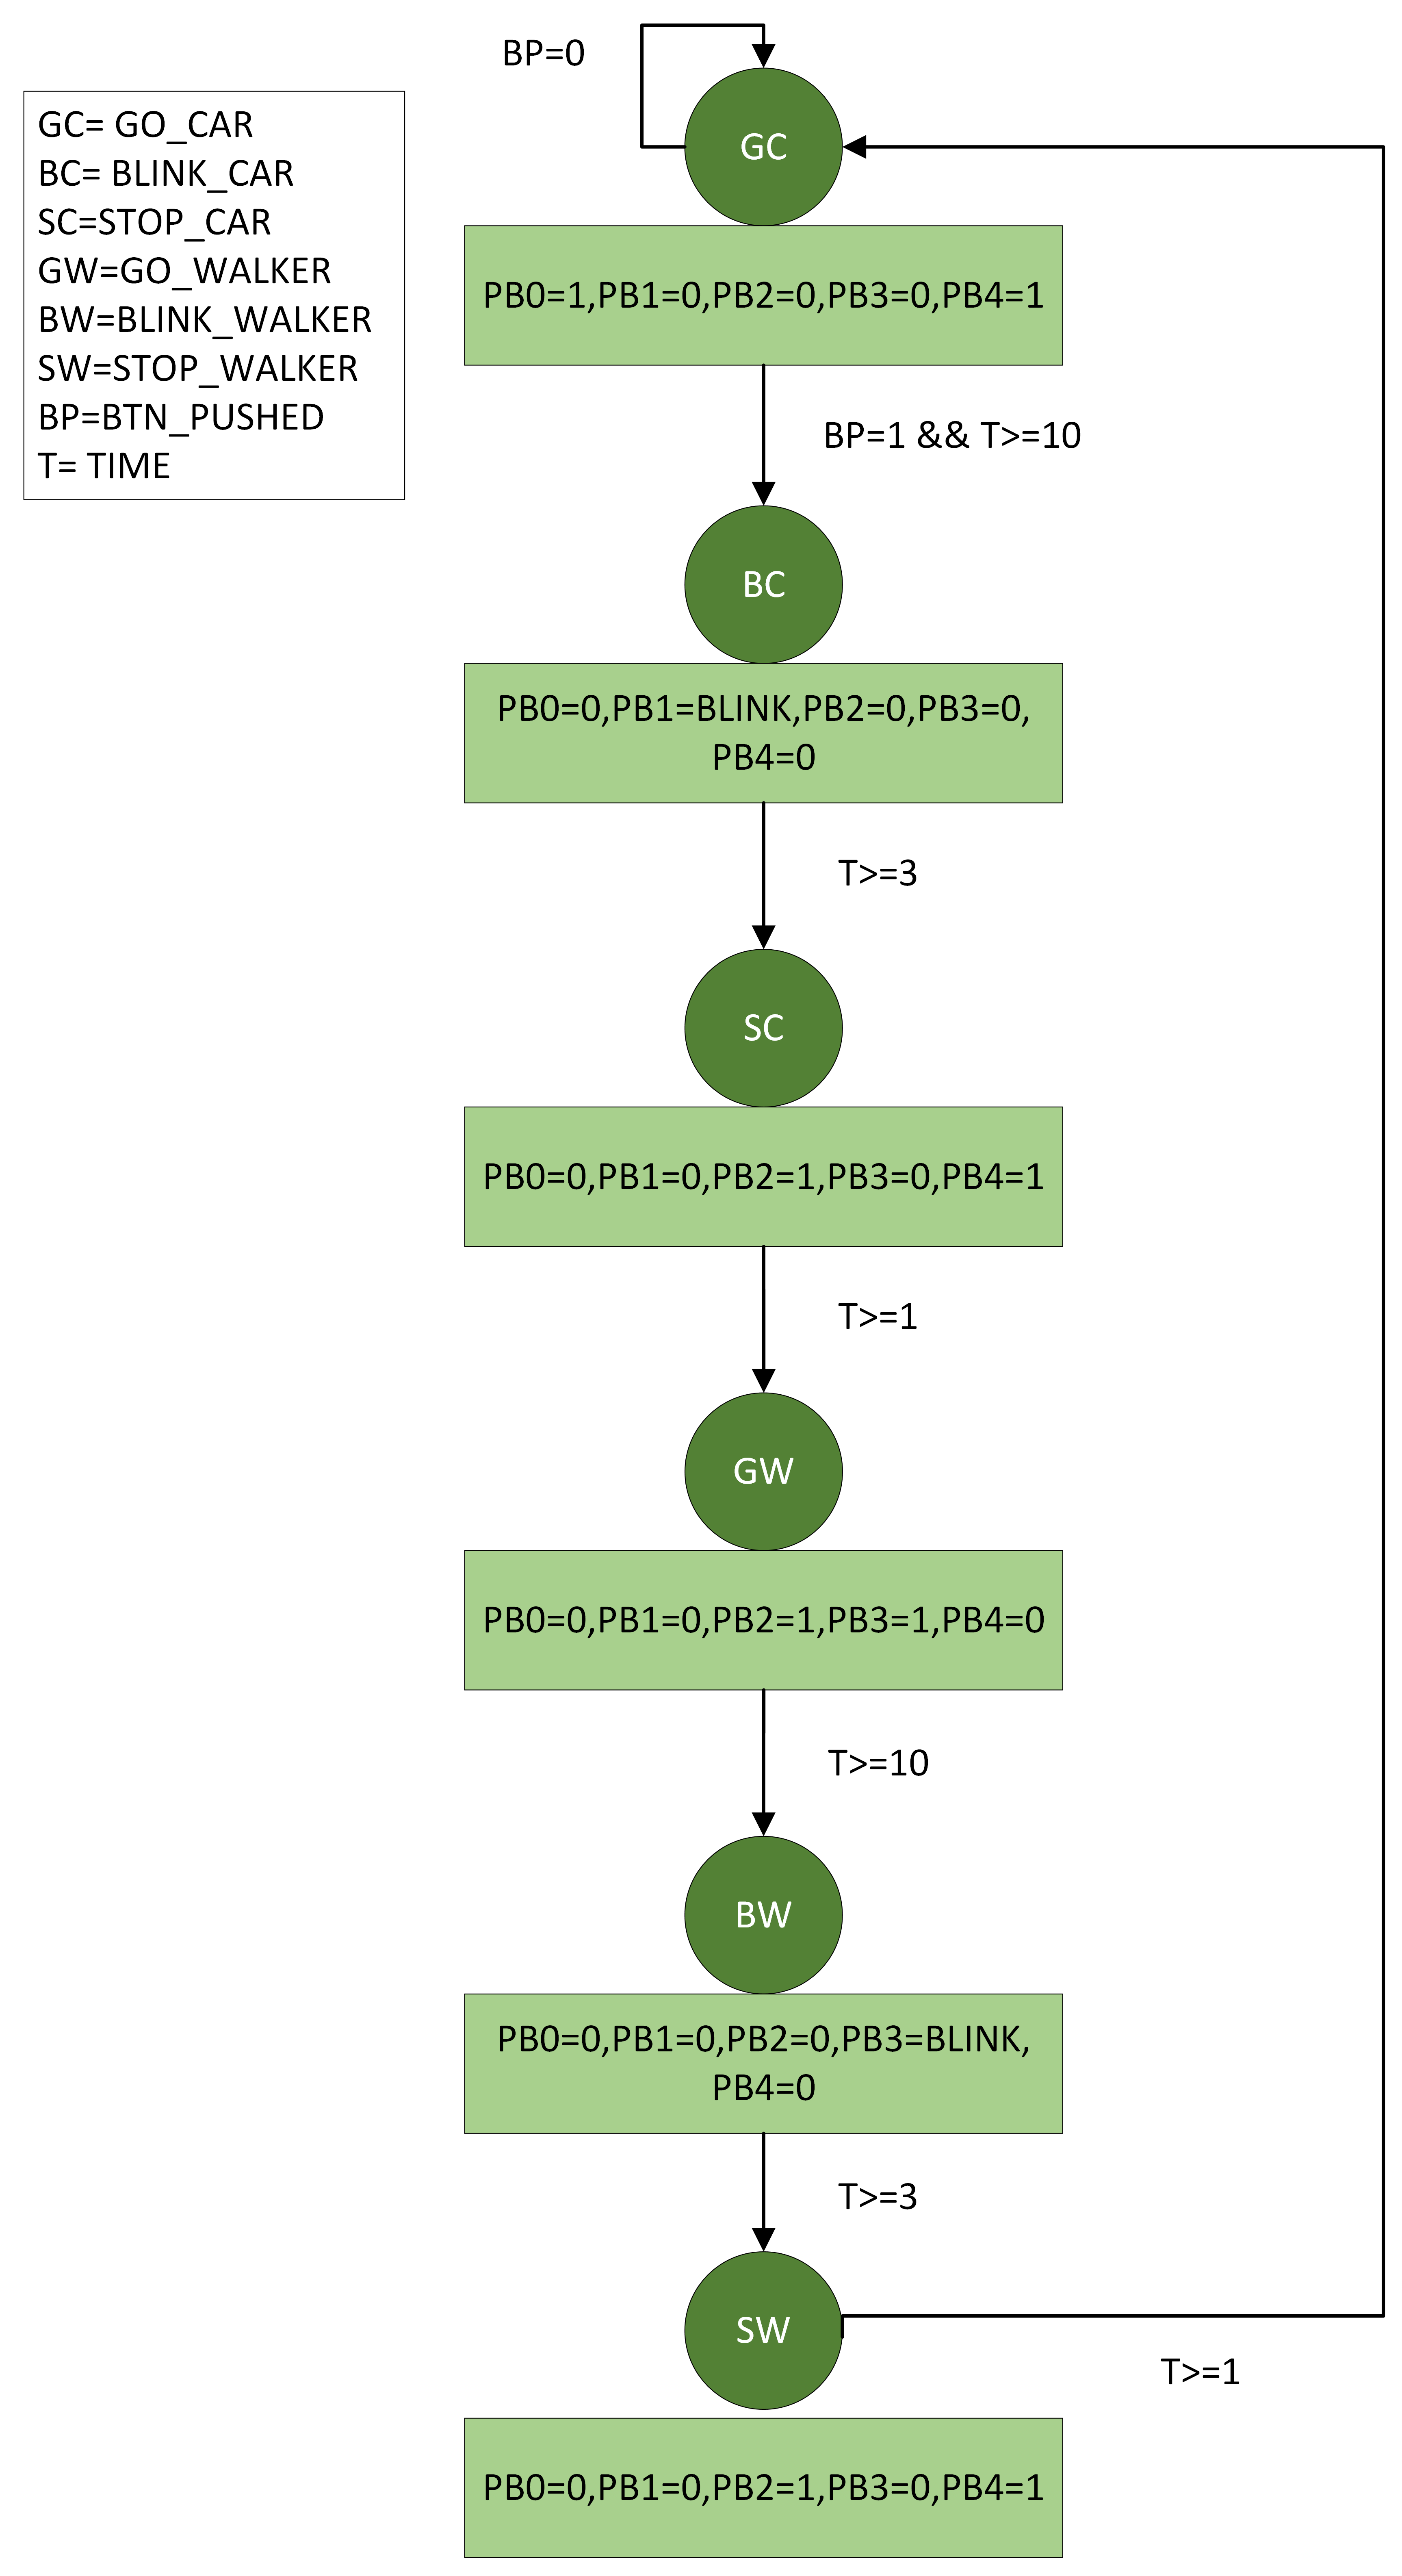
\includegraphics[scale=0.4]{./Figuras/Desarrollo_Analisis/Diagrama_Semaforo}
\caption{Diagrama FSM.}
\label{fig:FSMdiagram}
\end{figure}

\subsubsection{Función \texttt{main()}}
La función principal solamente hace el llamado de la función \texttt{init()} para configurar adecuadamente el ATtiny4313 y \texttt{FSM()} para iniciar con las transiciones de estado según sea el caso.  

\subsubsection{Construcción del circuito utilizado}
Para iniciar con la construcción de este circuito, es necesario tomar en cuenta los métodos de protección descritos en las secciones \ref{sec:cir0} y \ref{sec:cir1}. Una vez que ambos fueron unidos y construidos, se conectó la salida de este circuito al PD2 (pin 6 de la Figura \ref{fig:AT_pins}), ya que este se trata del pin encargado de detectar las interrupciones externas a través de INT0. El siguiente paso es la construcción de los semáforos. Los tres LED del semáforo vehicular necesitan de pines independientes, ya que su operación es distinta a la de los semáforos peatonales. En el caso de estos últimos, como su funcionamiento está sincronizado, sólo es necesario utilizar dos pines (uno para los LED verdes y otro para los rojos). Debido a la cantidad de pines necesarios, se selecciona el puerto B, es el que cuenta con la mayor cantidad de pines de I/O. El método de cálculo de las resistencias de cada LED puede observarse en la sección \ref{sec:cir2}. El circuito resultante tras implementar todas as consideraciones anteriores y utilizando \textit{tunnels} para hacer la disposición del circuito más clara, puede consultarse en la Figura \ref{fig:final}:

\begin{figure}[H]
\centering
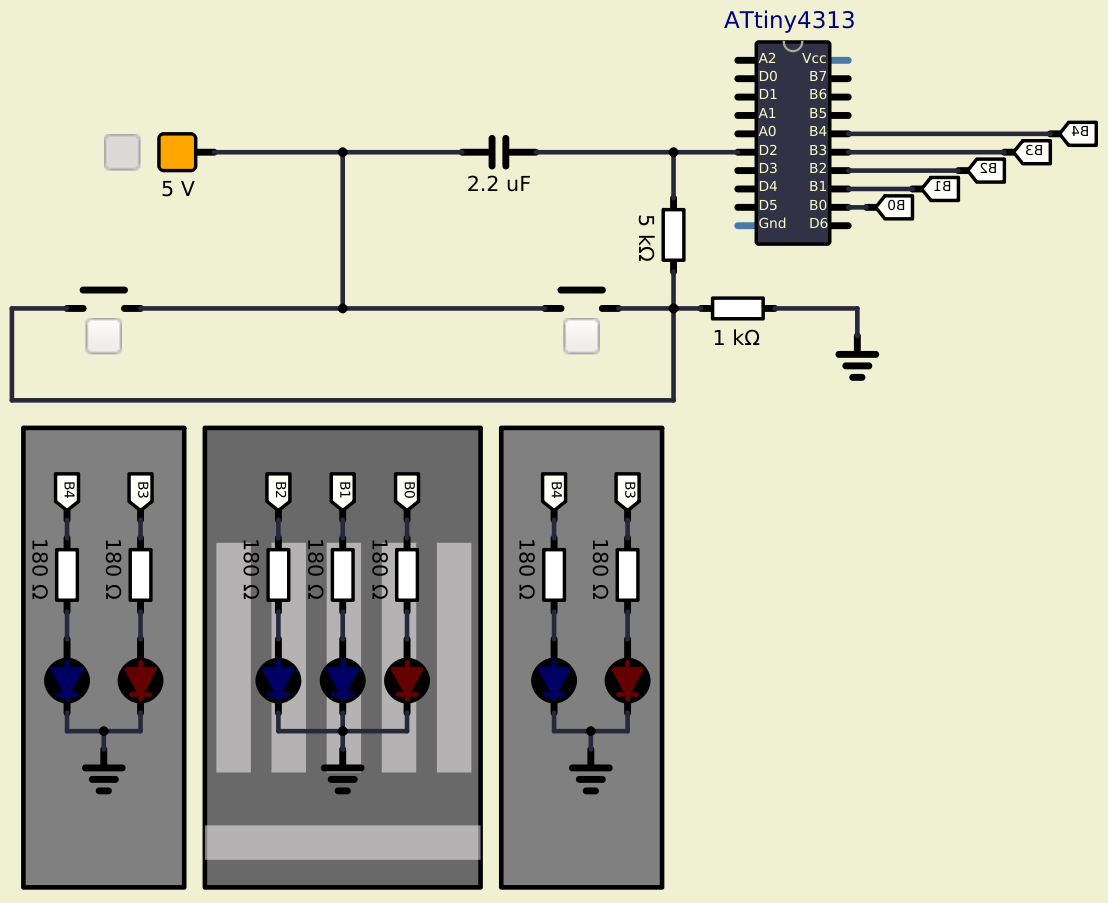
\includegraphics[width=125mm]{./Figuras/Desarrollo_Analisis/final}
\caption{Circuito final tras los cálculos de magnitudes y la implementación de las consideraciones necesarias.} 
\label{fig:final}
\end{figure}

\subsection{Análisis de los resultados}

\subsubsection{Funcionamiento del simulador del cruce peatonal según su estado}

A continuación se hará una demostración del funcionamiento de la simulación, mediante la demostración de cada uno de los 6 estados posibles de la FSM: 

\begin{itemize}
    \item Estado \textbf{\textit{GO\_CAR}} [0]: este corresponde al estado inicial y también es el estado por defecto. En este, la luz verde del semáforo vehicular y las rojas de los semáforos peatonales están encendidas. Los detalles pueden verse en la Figura \ref{fig:0}: 

    \begin{figure}[H]
    \centering
    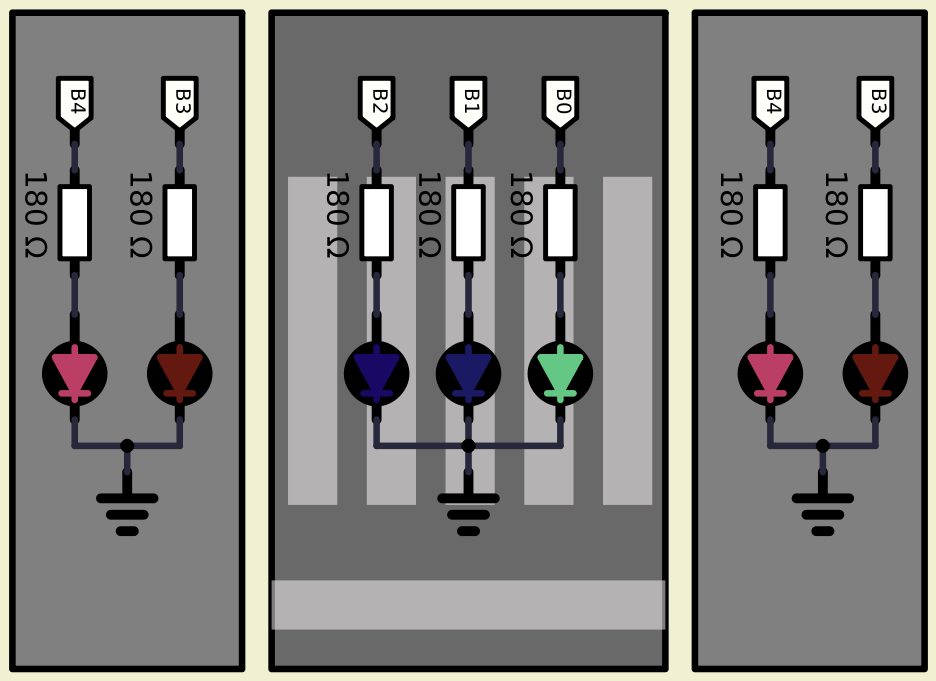
\includegraphics[width=95mm]{./Figuras/Desarrollo_Analisis/0}
    \caption{Estado GO\_CAR de la FSM.} 
    \label{fig:0}
    \end{figure}
    
    \item Estado \textbf{\textit{BLINK\_CAR}} [1]: en este estado la luz amarilla parpadea del semáforo vehicular parpadea, mientras que las luces rojas del semáforo peatonal están encendidas. Con las Figura \ref{fig:10} y \ref{fig:11} se muestra el parpadeo:

    \begin{figure}[H]
    \centering
    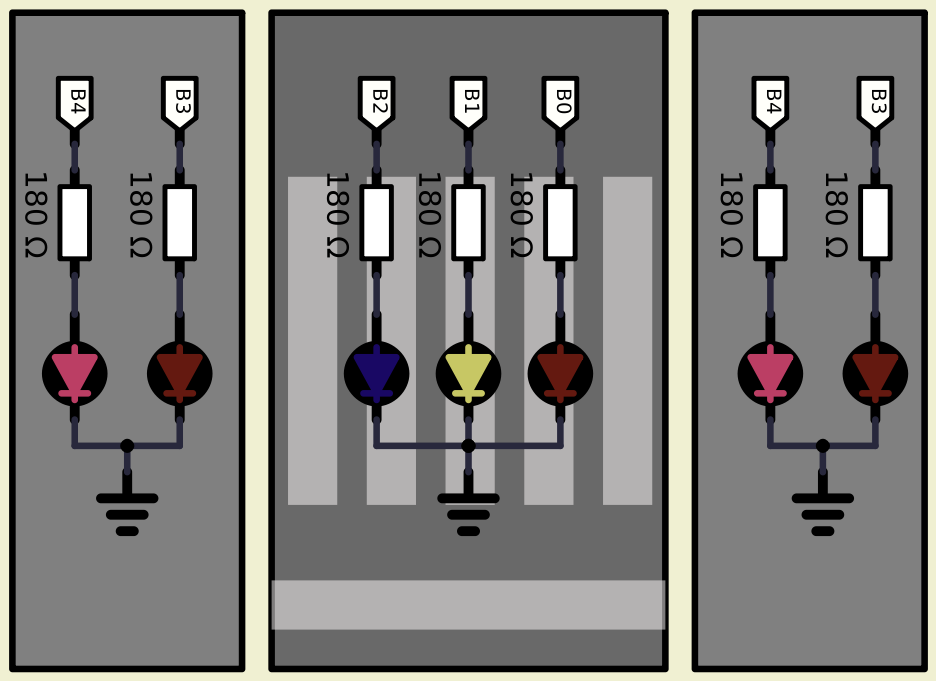
\includegraphics[width=95mm]{./Figuras/Desarrollo_Analisis/1_0}
    \caption{Estado BLINK\_CAR de la FSM, luz amarilla encendida.} 
    \label{fig:10}
    \end{figure}

    \begin{figure}[H]
    \centering
    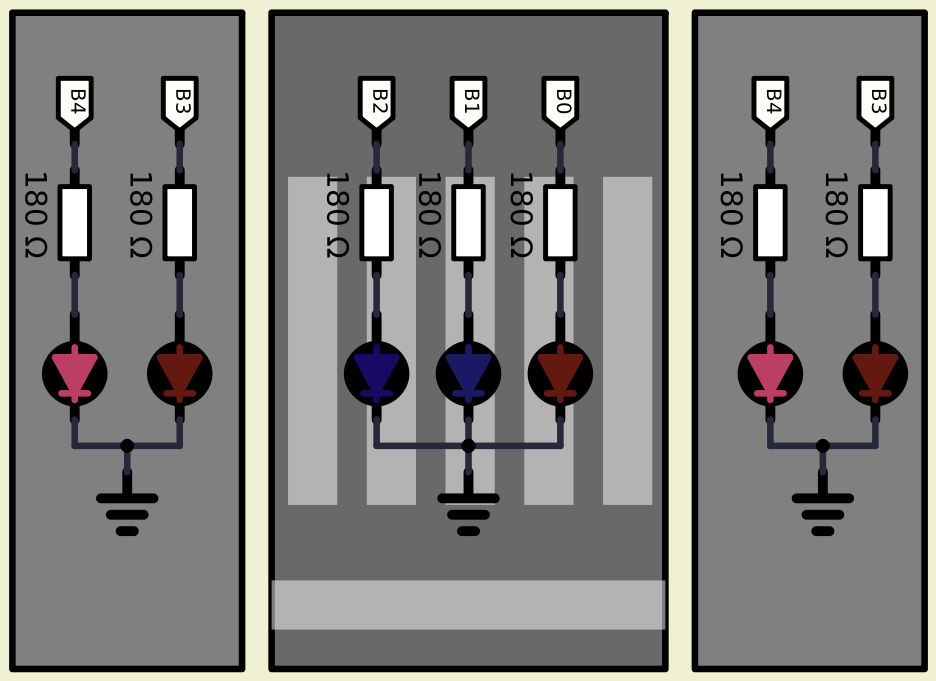
\includegraphics[width=95mm]{./Figuras/Desarrollo_Analisis/1_1}
    \caption{Estado BLINK\_CAR de la FSM, luz amarilla apagada.} 
    \label{fig:11}
    \end{figure}
    
    \item Estado \textbf{\textit{STOP\_CAR}} [2]: este corresponde un estado de transición en el que la luz roja del semáforo vehicular y las luces rojas del semáforo peatonal están encendidas al mismo tiempo. Los detalles pueden verse en la Figura \ref{fig:2}: 

    \begin{figure}[H]
    \centering
    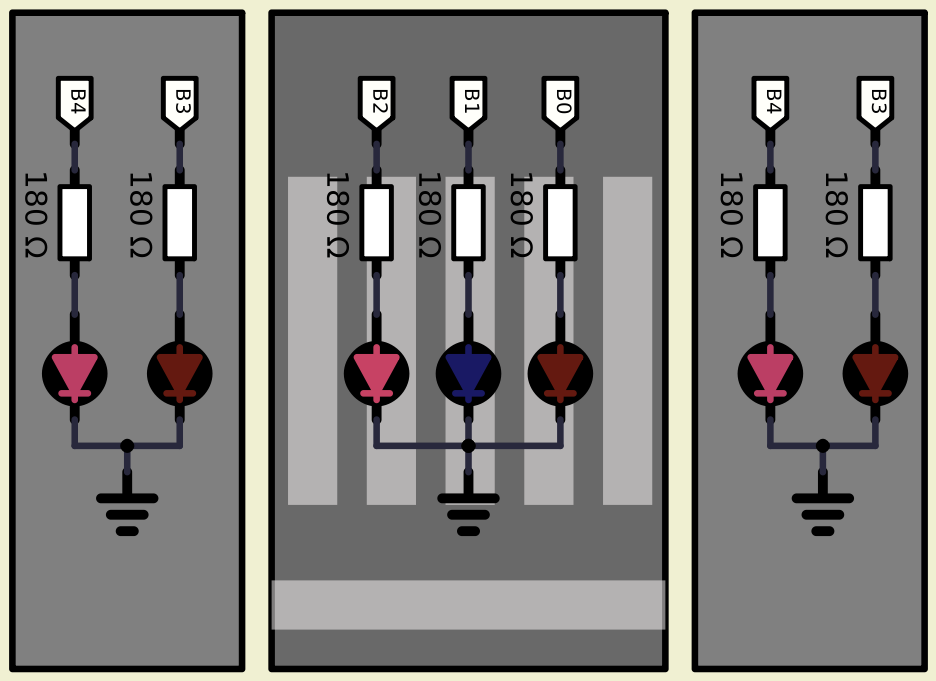
\includegraphics[width=95mm]{./Figuras/Desarrollo_Analisis/2}
    \caption{Estado STOP\_CAR de la FSM.} 
    \label{fig:2}
    \end{figure}
    
    \item Estado \textbf{\textit{GO\_WALKER}} [3]: en este estado, las luces verdes del semáforo peatonal y la luz roja del semáforo vehicular están encendidas. Los detalles pueden verse en la Figura \ref{fig:3}: 

    \begin{figure}[H]
    \centering
    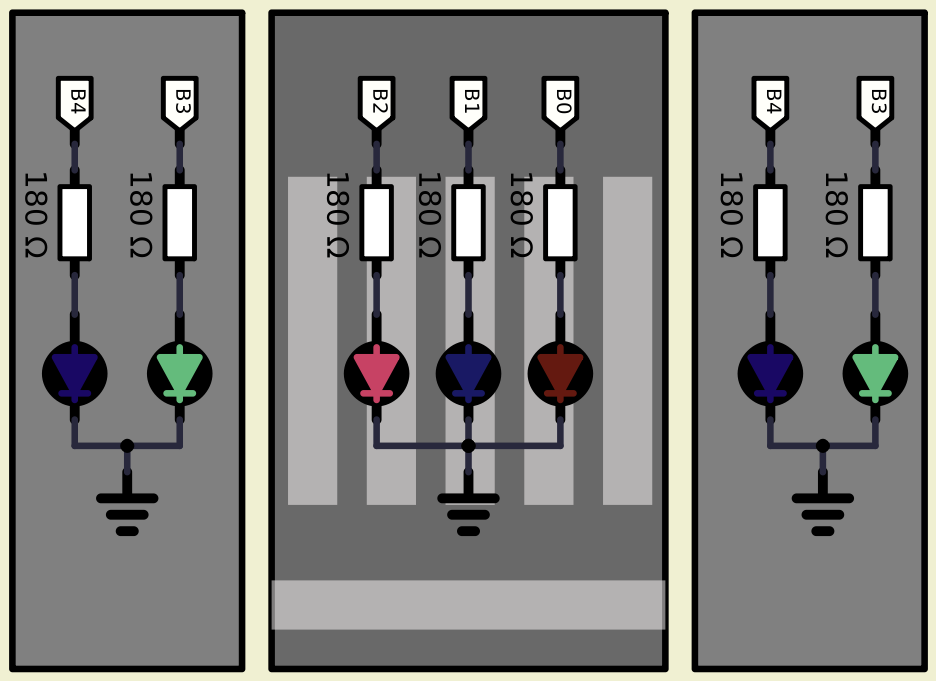
\includegraphics[width=95mm]{./Figuras/Desarrollo_Analisis/3}
    \caption{Estado GO\_WALKER de la FSM.} 
    \label{fig:3}
    \end{figure}
    
    \item Estado \textbf{\textit{BLINK\_WALKER}} [4]: en este estado las luces verdes del semáforo peatonal parpadean mientras la luz roja del semáforo vehicular está encendida. Con las Figura \ref{fig:40} y \ref{fig:41} se muestra el parpadeo:

    \begin{figure}[H]
    \centering
    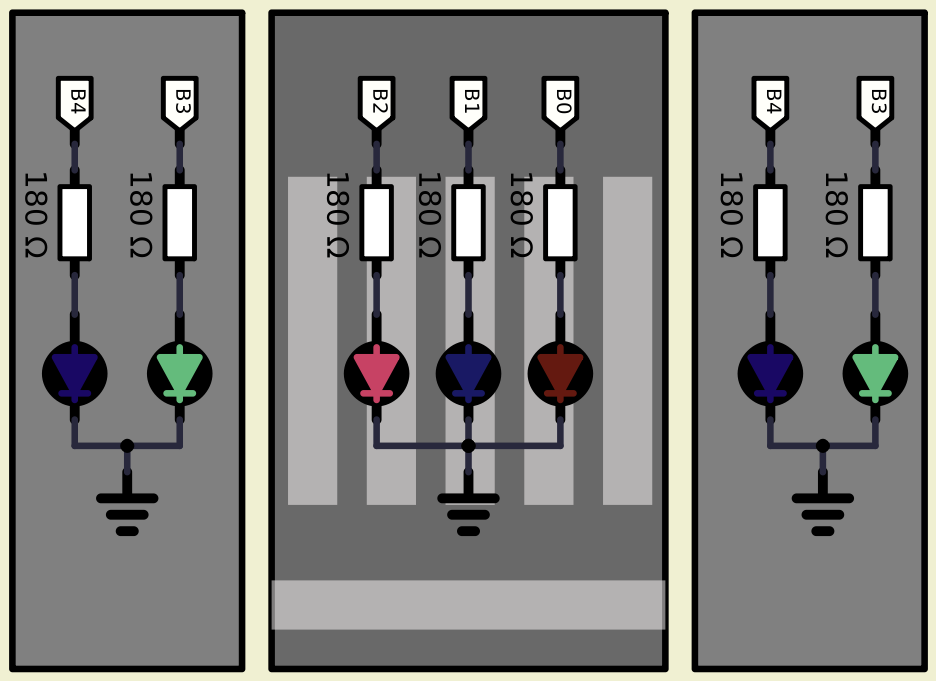
\includegraphics[width=95mm]{./Figuras/Desarrollo_Analisis/4_0}
    \caption{Estado BLINK\_WALKER de la FSM, luces verdes encendidas.} 
    \label{fig:40}
    \end{figure}

    \begin{figure}[H]
    \centering
    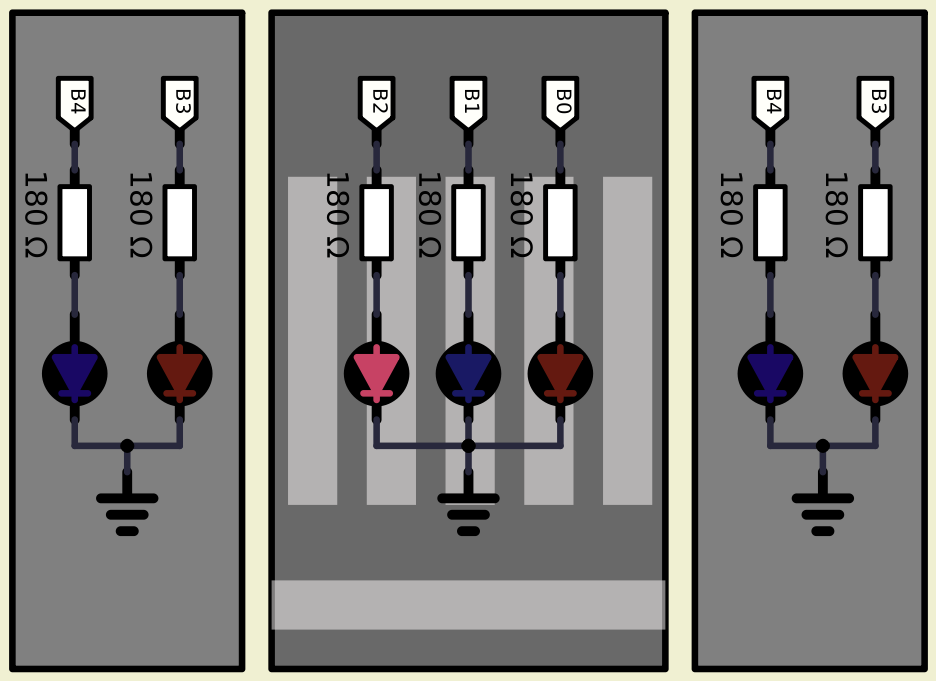
\includegraphics[width=95mm]{./Figuras/Desarrollo_Analisis/4_1}
    \caption{Estado BLINK\_WALKER de la FSM, luces verdes apagadas.} 
    \label{fig:41}
    \end{figure}
    
    \item Estado \textbf{\textit{STOP\_WALKER}} [5]: este corresponde un estado de transición en el que la luz roja del semáforo vehicular y las luces rojas del semáforo peatonal están encendidas al mismo tiempo. Los detalles pueden verse en la Figura \ref{fig:5}: 

    \begin{figure}[H]
    \centering
    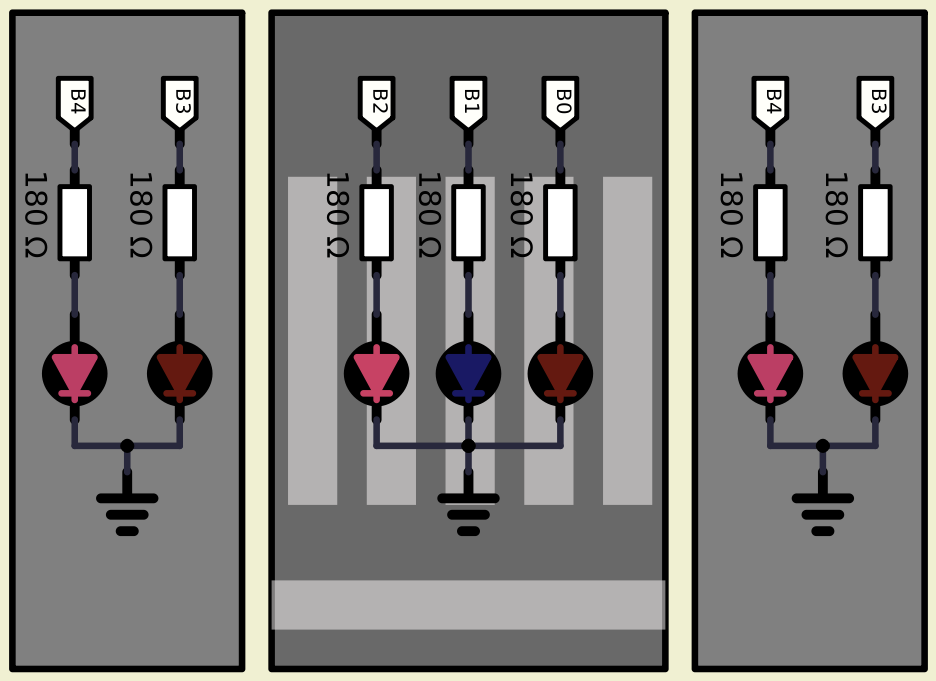
\includegraphics[width=95mm]{./Figuras/Desarrollo_Analisis/5}
    \caption{Estado STOP\_WALKER de la FSM.} 
    \label{fig:5}
    \end{figure}
\end{itemize}

Como puede observarse en las 6 figuras anteriores, los LED se encienden de manera adecuada según sea el estado en el que se encuentre el proceso. Para verificar el fila aleatoriedad de la implementación, se insta a la persona lectora del presente a probar la simulación por su cuenta. 

Una vez que el comportamiento a nivel de LED fue comprobado, puede analizarse también el comportamiento de la se señales obtenidas utilizando el osciloscopio. La configuración usada en el osciloscopio fué Time Div 2.5seg, Time pos 0.00ps y Volt div 500mV. 
 Las señales mostradas son:

\begin{itemize}
    \item LDPV: Luz de Paso Vehículos.
    \item LDPV-A: Luz de Paso Vehículos - Amarilla.
    \item LDVD: Luz de Vehículos Detenidos.
    \item LDPP: Luz de Paso de Peatones.
    \item LDPD: Luz de Peatones Detenidos.
\end{itemize}

En la Figura \ref{fig:ondas1} se muestra el inicio de la simulación, el estado iniciales (GO\_CAR), por lo que se puede esperar una LDPV y LDPD en alto, una LDPV-A,LDVD y LDPP en bajo esto se mantiene durante 10 segundos hasta que se acciona el botón. Inmediatamente al accionar se establece el siguiente estado (BLINK\_CAR), por lo que se puede observar como LDPV se coloca en bajo y la luz Amarilla comienza a parpadear durante 3 segundos, dando aviso a los conductores que la LDVD pronto se encenderá. 

%%%Primeros 10 segundos
\begin{figure}[H]
\centering
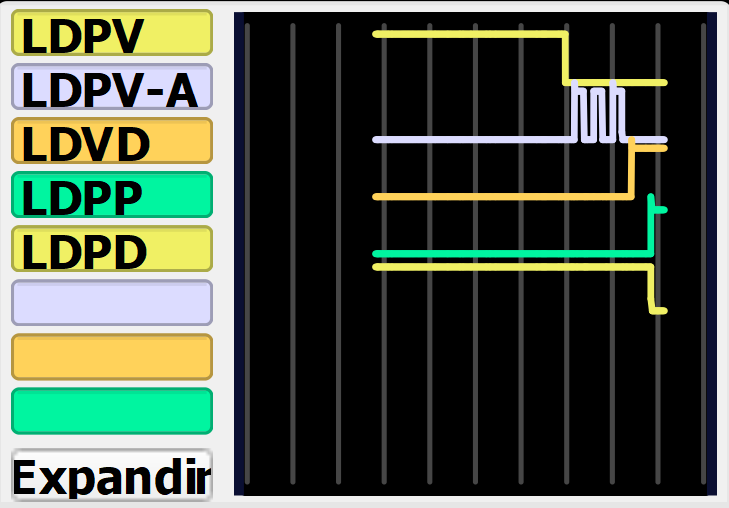
\includegraphics[width=95mm]{./Figuras/Desarrollo_Analisis/Primeros_10_segundos}
\caption{Análisis de ondas en Osciloscopio(Primeros 10 segundos).} 
\label{fig:ondas1}
\end{figure}
    
%%% Justo despues de 10 Segundos
Al terminar de parpadear LDPV-A, se pasa al siguiente estado (STOP\_CAR) coloca en alto LDVD y 1 segundo después se procede a encender la LDPP y apagar la LDPD (GO\_WALKER). En la Figura \ref{fig:ondas2} puede verse lo anterior:

\begin{figure}[H]
\centering
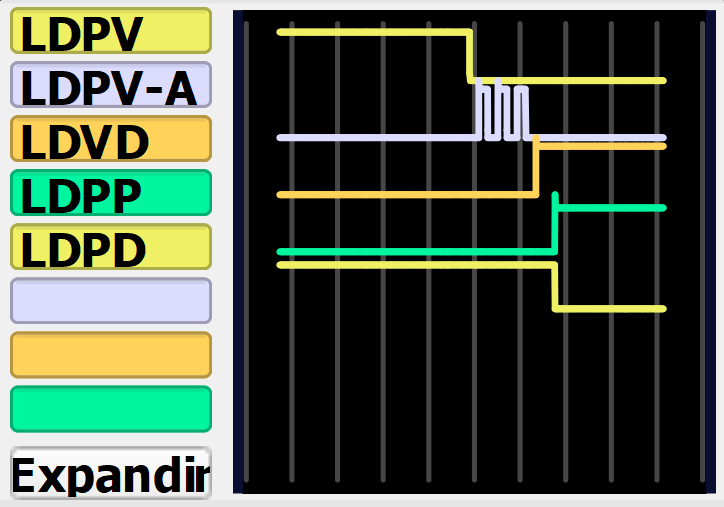
\includegraphics[width=95mm]{./Figuras/Desarrollo_Analisis/Luego_de_10_segundos_y_apretar_boton}
\caption{Análisis de ondas en Osciloscopio(Justo luego de 10 segundos).}
\label{fig:ondas2}
\end{figure}
    
Esta condición de pase de peatones se mantiene durante 13 segundos, sin embargo, al segundo 10 entra el estado (BLINK\_WALKER) y se procede a parpadear durante 3 segundos el led de LDPP indicando a los peatones que pronto se encenderá LDPD. Justo luego de parpadear entra el estado (STOP\_WALKER) se enciende LDPD y 1 segundo después entra el estado (GO\_CAR) se Apaga LDVD y de enciende LDPV de forma simultanea. En la Figura \ref{fig:ondas3} puede verse lo anterior:

%%% Ejecución completa
\begin{figure}[H]
\centering
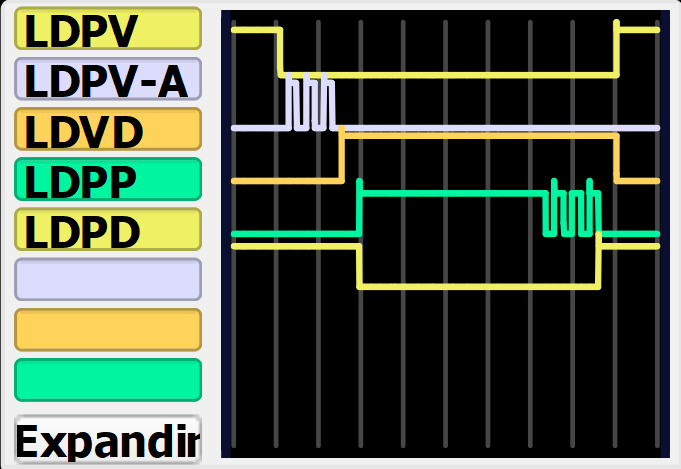
\includegraphics[width=95mm]{./Figuras/Desarrollo_Analisis/Ondas base}
\caption{Análisis de ondas en Osciloscopio(Completo).} 
\label{fig:ondas3}
\end{figure}

Finalmente, luego de este análisis de funcionamiento utilizando el osciloscopio, se puede decir que el funcionamiento cumple con el diagrama de temporización propuesto en el enunciado.